\documentclass[en]{../../../eplsummary}
\usepackage{tikz}
\usetikzlibrary{arrows, fit,automata, shapes,calc}
\tikzset{
    %Define standard arrow
    >=stealth',
    % Define arrow style
    pil/.style={
           ->,
           thick,
           shorten <=2pt,
           shorten >=2pt,}
}

\hypertitle{advSecu-lingi2144}{7}{lingi}{2144}
{Houtain Nicolas \and Kabasele Ndonda Gorby Nicolas}
{Gildas Avoine}

\section{Introduction}

\section{Vocabulary}

\begin{itemize}
    \item nonce: random number used only once
\end{itemize}


\section{Token-based Authentication}
\subsection{Definition}

\begin{description}
	\item[Identification:] We get the identity of a party
	\item[Authentication:] We get the identity of a party and the proof that the
	identity is true. The two parties are the \textbf{verifier}
    (verifies the proof) and the \textbf{prover} (provides the proof)
\end{description}

A token is an object that someone can own. They can be classified according to
technology used:

\begin{description}
	\item[Printed Tokens:] Tickets, Barcode
	\item[Digital Memory:] Magnetic strips cards,USB,\ldots
	\item[Microcircuit-based:] Smart cards,RFID,\ldots
\end{description}

\subsection{Printed Tokens}

    \paragraph{Human readable Tokens}
    \label{par:humanreadableTokens}

    \begin{itemize}
            \item When the ticket is provided by the verifier,
            the security is based on the difficulty to find the paper.
            \item When ticket printed on by the customer, forgery and
            copy can easy be detected.
    \end{itemize}

    \paragraph{Optically-readable Tokens}

    Data are represented such that it can be read by an optical
    machine. These token can be used for authentication.

\subsection{Digital-memory Tokens}

    For the magnetic stripe, sensitive data can be stored in the
    card or in a external database. Most magnetic stripe cards
    are \textsc{ISO-7811} compliant and contains 3 tracks.

\subsection{Microcircuits Tokens}

\begin{itemize}
    \item Classification on these tokens is done according to the
        calculation capabilities and the interface.
    \item Data can never leave the card,can be accessible after an
    authenfication and can be publicly accessible.
\end{itemize}

\section{RFID Primer}
\subsection{Definition}

\begin{description}
    \item[Radio Frequency IDentification:] Remotely retrieves data
    using devices called RFID tags through electromagnetic radiating
    waves.
    \item[RFID tags:] Small device containing a chip and an antenna to
    receive/respond to radio-frequency queries from an RFID reader/writer.
\end{description}
RFID tag can be low-capability device or porwerful contacless smartcard.
%%TODO Architecture slide 60?

\subsection{Daily Life Example}

\begin{itemize}
    \item Pet identification
    \item Localisation
    \item Book borrowing and inventories.
\end{itemize}

\subsection{Tags Characteristics}
\subsubsection{Power Source}
\begin{description}
    \item[Passive] Tags don't have any internal energy source. They
    get energy from the reader.
    \item[Active] Tags have a battery that is used both for internal
    calculations and transmission.
    \item[Semi-Passive] Tags only have energy for the calculation.
\end{description}


\subsubsection{Frequency Bands}
\begin{table}
    \centering
    \begin{tabular}{c|c|c}
        & Frequency & Range \\
        \hline
        Low Frequency &  124\text{-}135 kHz & centimeters \\
        High Frequency &  13.56 MHz & decimeters \\
        Ultra-High Frequency & 860\text{-}960 MHz & meters \\
    \end{tabular}
\end{table}

\subsubsection{Memory}
Tags have at least a few bits to store unique identifier UID\@.
\begin{itemize}
        \item UID size 32 to 128 bits.
        \item Usually, the UID is chosen by the manufacturer and cannot
        be changed by the user.
        \item EEPROM additional memory can be added (1KB or 70KB for passport)
\end{itemize}

\begin{description}
    \item[Tamper-resistance] A device is tamper-resistant if no adversary can
    get access to its protected memory by use of side-channel attacks.
    \item[Side-channel attack] An attack where the information is retrieved
    from physical implementation of a system (ex:Timing attack,physical attack).
\end{description}

\paragraph{Computation Capabilities}
The tags can perfom simple logic operation and symmetric/asymmetric
cryptographic. For symmetric cryptography, the microprocessor is not
necessarily needed.

\paragraph{Near Field Communication}
NFC is an extension of RFID, its main difference its that it offer
Peer-to-Peer connections between two (active) devices. NFC Data are exchanged
in a different format.

\subsection{Communication with the Tag}
For tags compliant with \textsc{ISO 7816}
\subsubsection{Memory}
Internal structure composed of files. There are two types of files:
\begin{itemize}
    \item Dedicated File (\textbf{DF})
    \item Elementary File (\textbf{EF}) that can be identified in two subtypes
    \begin{description}
        \item[Internal] Store information used by the card for management and
        control purpose.
        \item[External] Store information used exclusively by the outside world
    \end{description}
\end{itemize}
The Master File (\textbf{MF}) is a special \textbf{DF} and is the only mandatory
file. Each application is stored in a distinct \textbf{DF}.

Data inside an EF is stored in different formats:
\begin{description}
        \item[data unit] Smallest set of bits. Default value is 1 byte.
        \item[record] String of bytes which can be handled as a whole. Record
        can be referenced by a an 8-bit identifier.
        \item[date object] Structure of information which consists of a tag, a
        length and a value.
\end{description}

\paragraph{Communication}
The protocol used to exchange data is the Application Protocol Data Unit.

\section{Basic of Cryptography}
\subsection{Terminology}
\begin{description}
    \item[Cryptography] Science that design algorithms to ensure confidentiality
    of communication through insecure channels.
    \item[Confidentiality] Insurance that a given information cannot be accessed
    by unauthorized parties.
    \item[Cryptanalysis] Science that proves or disproves the security of
    cryptographic algorithm.
\end{description}
Break a cryptographic algortim means either:
\begin{itemize}
    \item Decrypting an encrypted message.
    \item Recovering the key of the cryptographic algorithm.
    \item Proving that a algorithm is less secure than what is claimed.
\end{itemize}

\paragraph{Attacker Model}
\begin{itemize}
    \item Adversary can be passive (ciphertext-only, known-plaintext) or
    \item active (chosen-plaintext,chosen-ciphertext)
\end{itemize}

\subsubsection{Encription Algorithm}
\begin{description}
    \item[Encryption algorithm] Algorithm that transforms an intelligible text
    into text that is unintelligible for non-authorized parties. The input is
    the plaintext and the output is the ciphertext.
\end{description}
Two categories of cryptographic algorithm:
\begin{itemize}
    \item Symmetric-key where the same key is used for both encryption and
    decryption.
    \item Asymmetric-key cryptography where there is a public key to encrypt and
    an private key to decrypt.
\end{itemize}

\subsection{Encryption}
%%TODO put it in table
\subsubsection{Symmetric-key Cryptography}
\begin{itemize}
    \item Based on bit or byte operations.
    \item Tend to be fast.
    \item Typical key-size: 128 bits
    \item Best attack is the exhaustive search.
\end{itemize}
Symmetric-key algorihtm can use Block ciphers or Stream ciphers. Block ciphers
acts on the plaintext in blocks. Stream ciphers acts on the plaintext one
symbol at a time.
\paragraph{Note:} DES is known to not be secure anymore.
\subsubsection{Asymmetric-key Cryptography}
\begin{itemize}
    \item Based on mathematical problems
    \item Best attack exploit the mathematical structure.
    \item Typical key size: 1024 bits.
    \item Encryptions and decryptions are slow.
\end{itemize}
\paragraph{Note:} RSA stands for Rivest-Shamir-Adleman
Certificate are used to identiry of the key owner. A Certificate authority
issue the certificate.

Parties can exchange their key or used Diffie-Hellman to agree on a shared key.

\subsection{Authentication and Integrity}
Entity authentication is asymmetric or symmmetric. Data authentication is
asymmetric or symmetric.

\subsection{Hash Function}
$$h:{0,1}*\rightarrow{0,1}^n$$
\begin{description}
    \item[First preimage resistance] Given a hash value y, it is infeasible to
    find m such that $h(m) = y$.
    \item[Second preimage resistance] Given a message $m_1$, it is infeasible
    to find a different message $m_2$ such that $h(m_1)=h(m_2)$.
    \item[Collision resistance] It is infeasible to find two different messages
    $m_1$ and $m_2$ such that $h(m_1)=h(m_2)$
    \item[Random oracle property] $h(m)$ is distinguishable from a random n-bit
    value.
\end{description}

\paragraph{Birthday Paradox} If we pick $\theta\sqrt{N}$ random numbers,
independently and uniformly, in {1,2,\ldots,N}, we get at least one number twice
with probability:
$$1-e^{-\frac{\theta^2}{2}}$$
With the Birthday paradox, we need about $\sqrt{2^n}$ hash operations to find a
collision with probability $\frac{1}{2}$
\paragraph{Message Authentication Code} Hash function that use a key.

\section{Authentication Protocols}
\subsection{Adversary Means}
\begin{description}
    \item[Eavesdropping] Adversary listens to the channel and hopes getting some
    useful data.
    \item[Skimming] Adversary queries the prover to get some useful information.
    \item[Modifying] Adversary modifies messages while they transit on the
    channel.
    \item[Injecting] Adversary injects messages on the channel.
    \item[Tampering] Adversary obtains content of the protected memory by
    physical means.
    \item[Exploiting] Adversary obtains information thanks to the system
    implementation.
    \item[Re-playing] Adversary replays a message she previously observed.
    \item[Pre-playing] Adversary plays the message she obtained.
    \item[Reflecting] Adversary reflects a reflect from a verifier so that
    answers itself.
    \item[Guessing] Adversary tries to guess the right answer or key w/o help of
    the prover.
    \item[Relaying] Adversary forwards the signal between ther verifier and the
    prover.
\end{description}
In the \textbf{Dolev-Yao} Model, adversary
\begin{itemize}
    \item Cannot guess random numbers
    \item Cannot decrypt or create valid ciphertexts without correct secret.
    \item Cannot retrieve private keys from public information.
\end{itemize}
\paragraph{Note:} To avoid replay and preplay attack, one-time password or
challenge/response protocol can be used.

%%TODO get schema from note
\subsection{One-time Passwords}
Password are generated with a one-way function.
\subsection{Challenge response}
Challenge response protocol can use different mechanism:
\begin{itemize}
    \item Timestamps where the challenge is based on clock.
    \item Sequence numbers where the challenge is based on hash on a
    one time password.
    \item Random numbers
\end{itemize}

%%Align all these
\subsection{ISO 9798 Challenge/Response}
ISO 9798\text{-}2 based on Symmetric-Key Encryption:
\begin{itemize}
    \item Mechanism-1
    		$$ A  \rightarrow B \quad E_k(t_A,B) $$
    \item Mechanism-2
    		$$ A  \leftarrow  B \quad r_B $$
    		$$ A  \rightarrow B \quad E_k(r_B,B) $$
    \item Mechanism-3
    		$$ A  \leftarrow B \quad r_B $$
    		$$ A  \rightarrow B \quad E_k(r_A,r_B,B) $$
    		$$ A  \leftarrow  B \quad E_k(r_n,r_A) $$
\end{itemize}
%%TODO VARIANT slide 162
ISO 9798\text{-}4 based on Hash function:
\begin{itemize}
    \item Mechanism-1
    $$ A \rightarrow B \quad H_k(t_A,B),t_A $$
    \item Mechanism-2
    $$ A \leftarrow B \quad r_B $$
    $$ A \rightarrow B \quad H_k(r_B,B),B $$
    \item Mechanism-3
    $$ A \leftarrow B \quad r_B $$
    $$ A \rightarrow B \quad H_k(r_A,r_B,B),r_A $$
    $$ A \leftarrow B \quad H_k(r_b,r_A,A) $$
\end{itemize}
ISO 9798\text{-}3 based on Public-Key Signature:
\begin{itemize}
    \item Mechanism-1
    $$ A \rightarrow B \quad S_A(t_A,B),B,t_A,cert_A $$
    \item Mechanism-2
    $$ A \leftarrow B \quad r_B$$
    $$ A \rightarrow B \quad S_A(r_A,r_B,B),B,r_A,cert_A $$
    \item Mechanism 3
    $$ A \leftarrow B \quad r_B $$
    $$ A \rightarrow B \quad S_A(r_A,r_B,B),B,r_A,cert_A $$
    $$ A \leftarrow B \quad S_B(r_B,r_A,A),A,cert_B $$
\end{itemize}
%%TODO VARIANT slide 174
\subsection{Authentication with Key Establshment}
During the phase of authentication phase, the two parties can exchange key
material.

ISO 11770\text{-}2 Symmetric-Key
\begin{itemize}
    \item Mechanism 4
    $$ A \leftarrow B \quad r_B $$
    $$ A \rightarrow B \quad E_k(r_B,B,k_1) $$
    The session key is $k_1$

    \item Mechanism 6
    $$ A \leftarrow B \quad r_B $$
    $$ A \rightarrow B \quad E_k(r_A,r_B,B,k_1) $$
    $$ A \leftarrow B \quad E_k(r_B,r_A,k_2) $$
    With a key-derivation function $f$, $f(k_1,k_2)$ is the session key.
\end{itemize}

Nedham\text{-}Schroeder Public-Key
\begin{itemize}
    \item Original Version
    $$ A \leftarrow B \quad P_A(k_1,B)  $$
    $$ A \rightarrow B \quad P_B(k_1,k_2) $$
    $$ A \leftarrow B P_A(k_2) $$
    $f(k_1,k_2)$ is the session key.
    \item Modified Version
    $$ A \leftarrow B \quad P_A(k_1,B,r_1) $$
    $$ A \rightarrow B \quad P_B(k_2,r_1,r_2) $$
    $$ A \leftarrow B \quad r_2 $$
\end{itemize}

ISO 11770\text{-} Asymmetric-Key
\begin{itemize}
    \item Mechanism 5
    $$ A \leftarrow B \quad r_B $$
    $$ A \rightarrow B \quad r_A,r_B,B,P_B(A,k_1),S_A(r_A,r_B,B,P_B(A,k_1))$$
    $$ A \leftarrow B \quad r_B,r_A,A,P_A(B,k_2),S_B,(r_B,r_A,A,P_A(B,k_2))$$
    Session key can be $f(k_1,k_2)$.
    \item Mechanims 6
    $$ A \leftarrow B \quad P_A(B,k_2,r_B) $$
    $$ A \rightarrow B \quad P_B(A,k_2,r_B,r_A) $$
    $$ A \leftarrow B \quad r_A $$
    Session key van be $f(k_1,k_2)$.
\end{itemize}
X.509
\begin{itemize}
    \item 2-Pass Mutual Authentication Protocol
    $$ A \leftarrow B \quad cert_B,D_B,S_B(D_B) $$
    $$ D_B = t_B,r_B,A,data*_1,P_A(k_1)* $$
    $$ A \rightarrow B \quad cert_A,D_A,S_A(D_A) $$
    $$ D_A = t_A,r_A,B,r_B,data_2,P_B(k_2)* $$
    $t_x$ defines a validity period and $r_x$ includes a sequential component.
    $f(k_1,k_2)$ is the session key.
    \item 3-Pass Mutual Authentication Protocol
    $$ A \leftarrow B \quad cert_B,D_B,S_B(D_B) $$
    $$ D_B = (t_B,r_b,A,data_1,P_A(k_1)*) $$
    $$ A \rightarrow B \quad cert_A,D_A,S_A(D_A) $$
    $$ D_A = (t_A,r_A,B,r_B,data*_2,P_B(k_2)*) $$
    $$ A \leftarrow B \quad r_A,A,S_B(r_A,A) $$
\end{itemize}

\section{Time-memory Trade-off}
\subsection{Motivations}

\paragraph{One-way Function} function $h:A \rightarrow B$, easy to compute but
hard to invert.
One-way function are used to store password. To break password, an exhaustive
search can be used in two different ways.
\begin{table}[ht!]
    \centering
    \begin{tabular}{c|c|c}
        & Online exhaustive search & Precalculated exhaustive search \\
        \hline
        Computation & $ |A|:=N $ & 0 \\
        Storage & 0 & N \\
        Precalculation & 0 & N \\
    \end{tabular}
\end{table}

\subsection{Hellman's TMTO}
Hellman table is used to precalculation phase to speed up the online attack.
\subsubsection{Table creation}
%$$ H: A \to B \quad the\ hash\ function $$
%$$ R: B \to A \quad the\ reduction\ function $$
%A number M of chains is generated from a arbitrary value in A\@:
\begin{tabular}{m{6cm}m{8cm}}
\begin{tikzpicture}

    \node[draw, circle] (A1) {S1};
    \node[draw, circle] (A2) [below=of A1] {};
    \node[draw, circle] (A3) [below=of A2] {};
    \node[draw, circle] (A4) [below=of A3] {E1};

    \node[draw, circle] (B1) [below right=0.5cm and 3cm of A1] {};
    \node[draw, circle] (B2) [below=of B1] {};
    \node[draw, circle] (B3) [below=of B2] {};

\node [draw, ellipse, fit={(A1) (A2) (A3) (A4)}] (F) {};
\node [draw, ellipse, fit={(B1) (B2) (B3) }] (FF) {};

\draw[->] (A1) edge node[above] {h} (B1);
\draw[->] (B1) edge node[above] {R} (A2);

\path[->] (A2) edge (B2)
(B2) edge (A3)
(A3) edge (B3)
(B3) edge (A4);

\end{tikzpicture}
&
\begin{itemize}
\item $h: A \to B$
\item $R: B \to A$

\item[$\Rightarrow$] R is the reduction function.
\end{itemize}
$$$$
\begin{tikzpicture}
    \node[draw, circle] (A1) {S1};
    \node[draw, circle] (A2) [right=of A1] {};
    \node[draw, circle] (A3) [right=of A2] {};
    \node[draw, circle] (A4) [right=of A3] {};

    \node[draw, circle] (A5) [right=of A4] {};
    \node[draw, circle] (A6) [right=of A5] {};
    \node[draw, circle] (A7) [right=of A6] {E1};

\path[bend left, ->] (A1) edge node[above] {h} (A2)
(A2) edge node[above] {R} (A3)
(A3) edge node[above] {h} (A4)

(A5) edge node[above] {h} (A6)
(A6) edge node[above] {R} (A7);

    \node[draw, circle] (B1) [below=of A1] {S2};
    \node[draw, circle] (B2) [right=of B1] {};
    \node[draw, circle] (B3) [right=of B2] {};
    \node[draw, circle] (B4) [right=of B3] {};

    \node[draw, circle] (B5) [right=of B4] {};
    \node[draw, circle] (B6) [right=of B5] {};
    \node[draw, circle] (B7) [right=of B6] {E2};

\path[bend left, ->] (B1) edge node[above] {h} (B2)
(B2) edge node[above] {R} (B3)
(B3) edge node[above] {h} (B4)

(B5) edge node[above] {h} (B6)
(B6) edge node[above] {R} (B7);

\end{tikzpicture}
\\
\end{tabular}
During the generation of the chains, chains may collide between each other, to
avoid that, different reduction function must be used.
\subsubsection{Online attack}
%%TODO ADD from the book, image
The idea is to take the a value $h$ in B, use the reduction function to get in A
and check if the value is contains in the last column of the table match.
If they don't match, use two reduction function and redo the verification.
If the verification fails, redo with 3 reduction function and so on.\ if
no match is found then the attack fails.

When there is a match, redo the chains from the beginning and stop when the
current value is equal to $h$. The password is the value just before $h$
%%TODO false alarms

\subsection{Oechslin Tables}
Oechslin tables also called rainbow table. The main difference compared to
Hellman table is that it uses different reduction function per column such that:

\begin{itemize}
    \item If 2 chains collide in different columns, they don't merge.
    \item If 2 chains collide in same column, merge can be detected.
\end{itemize}

\paragraph{Theorem} The success probability of a table is bounded:
\begin{itemize}
    \item
    Given $t$ and a sufficiently large $N$, the expected maximum number of
    chains per perfect rainbow table without merge is:
    $$ m_{\max}(t)\approx\frac{2N}{t+1} $$
    \item
    Given $t$, for any problem of size $N$, the expected maximum probability of
    success of a single perfect rainbow table is:
    $$ P_{\max}(t)\approx 1 - (1-\frac{2}{t+1})^t $$
    which tends toward $ 1 - e^{-2}\approx 86\% $ when $t$ is large.

    %%TODO have we seen that Average cryptanalysis time ?
\end{itemize}

\section{Generating Randomness}
\subsection{Introduction}
\begin{description}
    \item[Random Numbers] Random numbets are sequence of statistically
    independent and unbiased numbers.
    \item[Random Bits] Random bits are a sequence of statistically independent
    and unbiased binary digits.
    \item[Uniform distribution] All the numbers in a given range must occur
    equally often.
    \item[Independence] Given the knowledge of the all previous numbers
    generated, you can not predict the next number.
\end{description}

\subsubsection{Entropy}
The word entropy is used to describe a measure of randomness, a description
of how hard a value is to guess.
\begin{description}
    \item Let us assume that $X$ is a discrete random variable on the sample
    space $ \Omega_n = \{\omega_1,\omega_2,\ldots,\omega_n\} $ with the
    probability distribution $P=\{ p_i,1 \leq i \leq n \}$. The entropy $H(X)$
    of X is defined by:
    $$ H(X)= - \sum_{i=1}^{n} p_i \log_{2}p_i $$
\end{description}

\paragraph{Common Uses} Randomness is needed for key generation, nonces,salt,
\ldots

\subsection{Generating Randomness}
\begin{description}
    \item[Random bit Generator] A random bit generator is a device or algorithm
    which outputs a sequence of statistically independent and unbiased binary
    digits.
\end{description}

\paragraph{Note} A random integer in the interval [0;n] can be obtained by
generating a random bit sequence of length $ \lfloor \log{}{n} \rfloor + 1 $
and converting it to an integer.

\subsection{Hardware Random Number Generators}
The source of entropy come the software (time,process ID, user) or the hardware
(mechanical noises,electrical noises).

\subsubsection{Random Number Generators}
\begin{description}
    \item[Non-deterministic RNGs/True RNGs] Each bit produced by a HRNG comes
    from the observation of an unpredictable physical process.
    \item[Deterministic RNGs/PRNG] Each bit is produced by a deterministic
    algorithm properly initialized.
\end{description}

\subsection{PRNGs in Theory}
\begin{description}
    \item[Pseudo Random Bit Generator] A PRBG is a deterministic algorithm
    which given a truly random binary sequence of length k, outputs a binary
    sequence of length $l \gg k $ which 'appears' to be random. The input is
    the \textbf{seed}, while the output is the psedorandom bit sequence.
    \item[PRNG-FSM] A PRNG is a FSM defined by: $x_{t+1} = f(x_t)$.\ f is the
    transition function and $x_0$ is the seed.
    \item[Period] The period T of the PRNG is the smallest integer such that:
    $x_{t+T} = x_t$
\end{description}

\subsubsection{Middle-square Method}
To generate a sequence of n-digit pseudorandom numbers:
\begin{itemize}
    \item A n-digit seed is created and squared
    \item Middle n digits of the result are output and refeed the process
\end{itemize}
Example wiht n = 6
\begin{tikzpicture}
    \node (firstseed){847209};
    \node (textseed)[below=of firstseed,yshift=1cm] {seed};
    \node (result)[below=of textseed]{717\textcolor{red}{763089}681};
    \node (seedsquare) [below=of result,yshift=1cm]{$seed^2$};
    \node (result2)[below=of seedsquare]{763089};

    \draw[->] (textseed) -- (result);
    \draw[->] (seedsquare) -- (result2);
\end{tikzpicture}

\begin{itemize}
    \item For a generator of n-digits numbers, the period cannot be longer than
    $10^n$.
    \item If the middle n digits are all zeroes, the generator then outputs
    zeroes forever.
    \item If the first half of the middle n digits are all zeroes, the
    subsequent values decrease to zero.
    \item There exists short periods.
\end{itemize}

\subsubsection{Linear Congruential Generator}
\begin{description}
    \item[Linear Congruential Generator] A LCG produces a pseudorandom sequence
    of numbers $x_1,x_2,x_3,\ldots$ according to the linear recurrence:
    $$ x_n = a\times x_{n-1} + b \quad \mod{m}\quad with\ n \geq 1 $$
    The integers a (multiplier), b (increment), and m (modulus) are parameters
    which characterize the generatorn while $x_0$ is the (secret) seed.
\end{description}

\subsubsection{Blum-Blum-Shub Generator}
\begin{itemize}
    \item Let $m=p\times q$ where p and q are both primes congruent to 3 modulo
    4, and $ \gcd{\phi(p)}{\phi(q)} $ is small.
    \item Let $x_0$ be a seed.
    \item We iterate $x_{n+1} := x^2_n\ \mod{m}$
    \item We output the parity bit of $x_n$ (n>0).
    %TODO Comment
\end{itemize}

\subsubsection{ANSI X9.17}

\begin{itemize}
    \item Input: a random (and secret) 64-bit seed $x_0$, integer m, and a
    DES E-D-E encryption key k.
    \item Output: m pseudorandom 64-bit string $x_1,x_2,\ldots,x_m$
    \begin{enumerate}
        \item $T_t = E_k(time())$
        \item $o_t = E_k(x_t \oplus T_t)$
        \item $x_{t+1} = E_k(T_t \oplus o_t)$
    \end{enumerate}
\end{itemize}

\subsubsection{LFSR}
\begin{figure}[ht!]
    \centering
    \begin{tikzpicture}
        \node [shape = rectangle](b3) {b3};
        \node [shape = rectangle, right=of b3] (b2) {b2};
        \node [shape = rectangle, right=of b2] (b1) {b1};
        \node [shape = rectangle, above=of b1] (xor) {$\oplus$};
        \node [shape = rectangle, right=of b1] (b0) {b0};
        \node [above of=b0](xoranchorr){};
        \node [above of=b3](xoranchorl){};

        \draw [->] (b3) -- (b2);
        \draw [->] (b2) -- (b1);
        \draw [->] (b1) -- (b0);
        \draw [->] (b1) -- (xor);
        \draw (b0) -- (xoranchorr);
        \draw [->] (xoranchorr) -- (xor);
        \draw (xor) -- (xoranchorl);
        \draw [->] (xoranchorl) -- (b3);
    \end{tikzpicture}
\end{figure}

\section{Implementation of Hash Functions}
\subsection{Common Hash Functions}
\begin{itemize}
    \item Output size:
    \begin{itemize}
        \item MD5: 128bits
        \item SHA-1: 160 bits
        \item SHA-2: 224/256/384/512 bits
        \item RIPEMD:\@160/128/256/320 bits
        \item Whirlpool: 512 bits
    \end{itemize}
    \item Input size:
    \begin{itemize}
        \item In theory, the size is unlimited but in pratice it is limited
        because the length of the message is concatenated at the end of it and
        follows a predefined format
        \item Internal function with small input size sequentially iterated on
        blocks of messages.
    \end{itemize}
\end{itemize}

\subsection{An insider view}
%%TODO complete
\begin{figure}[ht!]
    \centering
    \begin{tikzpicture}
        \node (input){arbitrary length input};
        \node [shape=rectangle,below =of input](preprocessing){data preprocessing};
        \node [shape=rectangle,below =of preprocessing](compression)
        {compression function};
        \node [shape=rectangle,below =of compression](transformation)
        {optional transformation};
        \node [below =of transformation](output){fixed length output};

        \draw [->] (input) -- (preprocessing);
        \draw [->] (preprocessing) -- (compression);
        \draw [->] (compression) -- (transformation);
        \draw [->] (transformation) -- (output);
    \end{tikzpicture}
\end{figure}

\subsection{Conclusion}
\begin{table}
    \centering
    \begin{tabular}{c|c|c|c}
        Primitive & Output Length & Legacy & Future \\
        \hline
        SHA-2 & 224,256,384,512 & Yes & Yes \\
        SHA-3 & TBA & Yes & Yes \\
        Whirlpool & 512 & Yes & Yes \\
        \hline
        RIPEMD-160 & 160 & Yes & Yes \\
        SHA-1 & 160 & Yes & No \\
        \hline
        MD-5 & 128 & No & No \\
        RIPEDMD-128 & 128 & No & No \\
    \end{tabular}
\end{table}

\section{Implementation of Block Ciphers}
\subsection{Choice of the Block Cipher}
\begin{table}
    \centering
    \begin{tabular}{c|c|c}
        Primitive & Legacy & Future \\
        \hline
        AES & Yes & Yes \\
        Camelia & Yes & Yes \\
        \hline
        Three-key-3DS & Yes & No \\
        Two-key-3DS & Yes & No \\
        Kasumi & Yes & No \\
        Blowfish & Yes & No \\
        \hline
        DES & No & No\\
    \end{tabular}
\end{table}

\subsection{Key Generation}
Some block ciphers suffer from poor keys. For example DES has 16 known poor
(weak and semi-weak) keys. %TODO add definition

\subsection{Mode of Operation} %TODO add schema
Mode of operation is used to define how to encrypt a message whose length
is larger than the cipher block size.
\subsubsection{Electronic codeBook}

\begin{itemize}
    \item Block oriented
    \item Require padding
    \item Do not require initialization vector.
    \item Parallel encryption possible and parallel decryption possible.
    \item Swapping blocks is undetectable
    \item Same plaintext blocks produce same ciphertext blocks
    \item Not suitable for long or strongly structured messages
\end{itemize}

\subsubsection{Cipher Block chaining}

\begin{itemize}
    \item Block oriented
    \item Require padding
    \item Require initialization vector
    \item Parallel encryption not possible but parallel decryption possible
    \item General-purpose block-oriented encryption
\end{itemize}

\subsubsection{Cipher feedback}

\begin{itemize}
    \item Stream-oriented
    \item Do not require padding
    \item Require initialization vector
    \item Parallel encryption not possible but decryption possible (if IV known)
    \item Decryption can be done with the encryption function
    (cannot be used with a PK cipher)
    \item General-purpose stream-oriented encryption
\end{itemize}

\subsubsection{Output feedback}

\begin{itemize}
    \item Stream-oriented
    \item Do not require padding
    \item Require initialization vector
    \item Prepocessing possible for encryption and decryptio (if IV known)
    \item Decryption can be done with encryption function
    (cannot be used with a PK cipher)
    \item Enable preprocessing
\end{itemize}

\subsubsection{Counter}

\begin{itemize}
    \item Stream-oriented
    \item Do not require padding
    \item Do not require initialization vector
    \item Preprocessing possible for encrytion and decryption
    (nonce/counter known)
    \item Decryption can be done with encryption function. (cannot not be used
    with a PK cipher)
    \item Same as OFB but randomizes the encryption with a counter value instead
    of some feedback from previous blocl
    \item Must have a different counter value for every plaintext block.
    \item Enable preprocessing, Random access.
\end{itemize}

\subsection{Initialization Vector}
Required with CBC,CFB,OFB %%TODO complete with note

\subsection{Padding}
\begin{itemize}
    \item Main aim of padding is to fill the last block of plaintext (No
    necessarily the shortest)
    \item Can be eithet bit vs byte-oriented
    \item Required with ECB and CBC
    \item Padding should be checked after decryption
    \item Padding increases the size of the plaintext
\end{itemize}

\subsubsection{ISO/IEC 9797}
\begin{itemize}
    \item Method 1: Append some 0-bits (possibly none) to the end of the message
    to fill the last block of plaintext. Problem is that it brings ambiguity if
    recipient does not know the length of the plaintext.

    \item Method 2: Put a 1-bit at the end of the plaintext, then pad with
    some 0-bits (possibly none) to fill the last block of plaintext. To avoid
    ambiguity, plaintext should always be padded even if the last block is
    already completed.
\end{itemize}

\subsubsection{ANSI X9.23}
Append some 0-bits to the message and the length (in bytes) of the padding.

\subsubsection{ISO/IEC 10126}
Append some random bits to the message and the length (in bytes) of the padding.

\subsubsection{PKCS 7}
Each added byte is the length (in bytes) of the padding.

\subsection{Cipher used as Hash Function}
A block cipher can be used in place of a hash function.
\paragraph{Davies-Meyer} $H_i=E_{m_i}(H_{i-1})\oplus H_{i-1}$ The $m_i$ are
blocks of the padded message to be hashed. This construction leads to fixed
points $E_m(h)\oplus h=h$.
\paragraph{Matyas-Meyer} $h_i = E_{g(H_{i-1})}(m_i)\oplus m_i$
\begin{itemize}
    \item $m_i$ are blocks of the padded message to be hashed.
    \item Function g is just to map the output size of H into the key size.
\end{itemize}

\section{Implementation of Stream Ciphers}
\subsection{Basics}
\begin{table}
    \centering
    \begin{tabular}{c|c|c}
        Primitive & Legacy & Future\\
        \hline
        Rabbit & Yes & Yes\\
        SNOW3G & Yes & Yes\\
        \hline
        Trivium & Yes & No\\
        SNOW2.0 & Yes & No\\
        \hline
        RC4 & No & No\\
    \end{tabular}
\end{table}

\paragraph{One-Time Pad} $C_i = M_i \oplus K_i\quad for\ i=1,2,3,\ldots$
\begin{itemize}
    \item Key must be generated randomly
    \item Key must be at least as long as the message
    \item Key must be used once
\end{itemize}
A stream ciphers deal with these drawbacks
\begin{itemize}
    \item Key!= Keystream, keystream is generated pseudo-randomly
    \item Key is shorter than the message
    \item Key cannot be used more than once: An IV is appended to the key to
    counter this problem.
\end{itemize}
As with block ciphers, stream ciphers do not ensure integrity (Associativity
and commutativity)

\begin{itemize}
    \item Synchronized mode
    \begin{itemize}
        \item Use a single long stream during the session
        \item A and B initialize the stream with the shared key
        \item A uses the first $|m_A|$ bits of the stream to encrypt message
        $m_A$
        \item B uses the next $|m_B|$ bits of the stream to encrypt message
        $m_B$
    \end{itemize}

    \item Unsynchronize mode
    \begin{itemize}
        \item The keystream is reinitialized for each new packet
        \item Initialization depends on two inputs k and IVi\@.
        \item k secret but constant key
        \item IV non-secret but changing initial vector
    \end{itemize}
\end{itemize}

\subsubsection{Linear Feedback Shift Registers}
\paragraph{Linear feedback shift register} LFSR\footnote{see section random}
of length L consists of L
stages numbered 0,1,\ldots,L-1, each capable of storing one bit and having one
input and one output; and a clock which controls the ovements of data.

During each init of time the following operations are performed:
\begin{itemize}
    \item The content of stage 0 is outputed and forms part of the output
    sequence.
    \item The content of stage i is moved to stage i-1 for each i,
    $1\leq i\leq L-1$
    \item The new content of stage L-1 is the feedback bit $s_j$ which is
    calculated by adding together modulo 2 the previous contents of a fixed
    subsets of stages 0,1,\ldots,L-1.
\end{itemize}
LFSR should never be used by itself as keystreamn generator but they have the
advantage of having low implementation costs. To destroy the linearity:
\begin{itemize}
    \item A nonlinear combining function on the outputs of several LFSRs
    \item A nonlinear filtering function on the contents of a single LFSR
    \item The output of one (or more) LFSRs to control the clock of one
    (or more) other LFSRs.
\end{itemize}

\subsection{RC4}
Use a secret key of length from 1 to 256 bytes.

\subsection{Conclusion}
Using a stream cipher is tricky as the security of stream ciphers is not
well-established, therefore it should be used carefully.

\section{Implementation of Message Authentication Code}
\subsection{Basics}
The goal of MAC is to prevents tampering with a message. MAC require a secret
key otherwise modification of the message cannot be done. MAC ensures integrity,
authentication but not confidentiality.

\subsection{Constructions}
Let h be a hash function, k a key, m the message to be MACed, and M the
computed MAC\@.
\begin{itemize}
    \item Prefix method: $ M = h(k||m) $
    \item Suffix method: $ M = h(m||k) $
    \item Envelop method:$ M = h(k||p||m||k) $
\end{itemize}
MAC uses hash function rather than block cipher because hash function are
generally faster.
\begin{figure}[ht!]
    \centering
    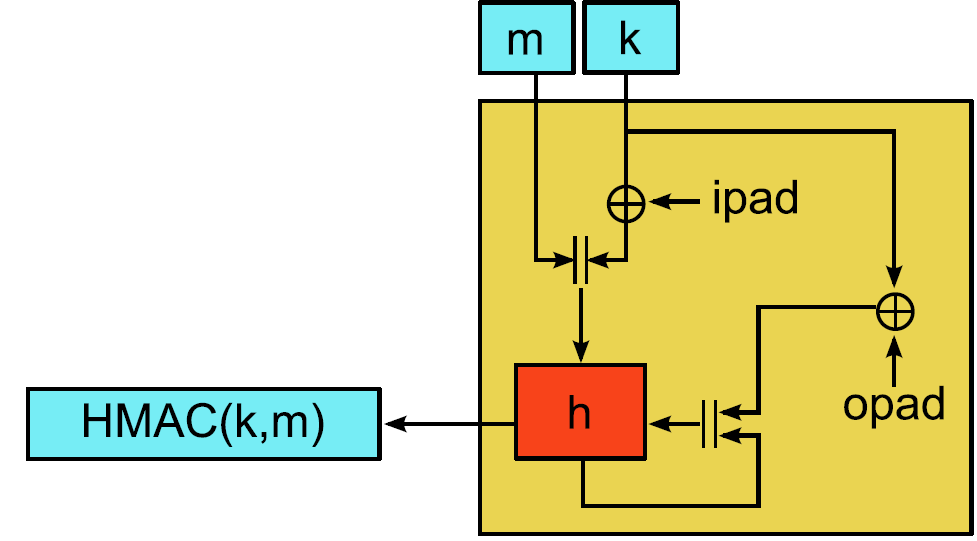
\includegraphics[scale=0.5]{img/hmac}
\end{figure}

\subsubsection{Built upon a cipher}
Based on the CBC mode of operation
\begin{itemize}
    \item The message is encrypted in CBC mode
    \item Final block is the MAC
    \item Intermediary blocks are thrown out
    \item IV consists of zeros
\end{itemize}

\begin{figure}[ht!]
    \centering
    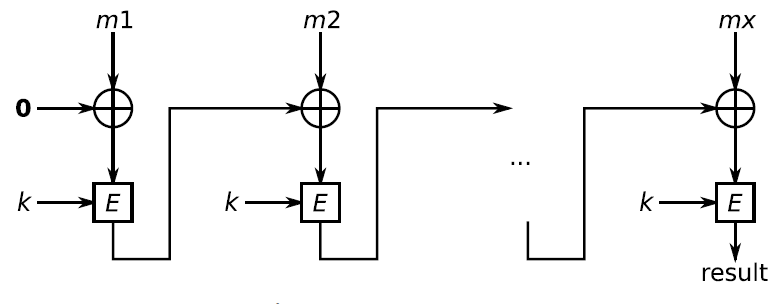
\includegraphics[scale=0.5]{img/cbc-mac}
\end{figure}

\begin{itemize}
    \item CBC-MAC is secure for messages of a fixed number of blocks assuming
    the block cipher is secure.
    \item Not secure with variable lengths
    \item CBC-MAC $(length(M)||M)$ to avoid truncation attacks
    \item Encrypt $length(M)$ with K, yielding K' and use it as key for the
    MAC function
\end{itemize}
\paragraph{Note:} There is a improvement of CBC-MAC known as Retail-MAC where
the last block is decrypted with key k' then re-encrypted with k. This reduces
the threat of exhaustive key search
\begin{itemize}
    \item The IV should not be random
    \item Slower than HMAC
    \item The MAC can be truncated to enforce security but this also reduces the
    key search space
\end{itemize}

\subsection{Encrypt and MAC}
Encryption does not ensure integrity but MAC does, so they must be combined.
From the \textbf{LESS} to the \textbf{STRONGER} security:
\begin{itemize}
    \item $ E_K(M) $
    \item Redundancy-then-Encrypt: $ E_K(M,R(M)) $
    \item Hash-then-Encrypt: $ E_K(M,h(M)) $
    \item Hash and Encrypt: $ E_K(M),h(M) $
    \item MAC and Encrypt: $ E_{h1(K)},MAC_{h2(K)}(M) $ (SSH)
    \item MAC-then-Encrypt: $ E_{h1(K)}(M,MAC_{h2(K)}(M)) $ (SSL)
    \item Encrypt-then-MAC\@: $ E_{h1(K)}(M),MAC_{h2(K)}(E_{h1(k)}(M)) $ (IPSec)
\end{itemize}
\paragraph{Note:} Do not hash concatenation of key and message to get a MAC\@.
Never use the same key for both encryption and MAC\@.

\section{Relay attack and Countermeasures}
\subsection{Relay attacks}
\begin{description}
    \item[Relay Attack] A relay attack is a form of man-in-the-middle where the
    adversary manipulates the communication by only relaying the verbatim
    messages between two parties.
    \item[Man-In-The-Middle Attack] A man-in-the-middle (MITM) us a form of
    attack, where the adversary provokes or manipulates the communication
    between two parties. Manipulating the communication means relay, withold, or
    insert messages.
\end{description}

\begin{figure}[ht!]
    \centering
    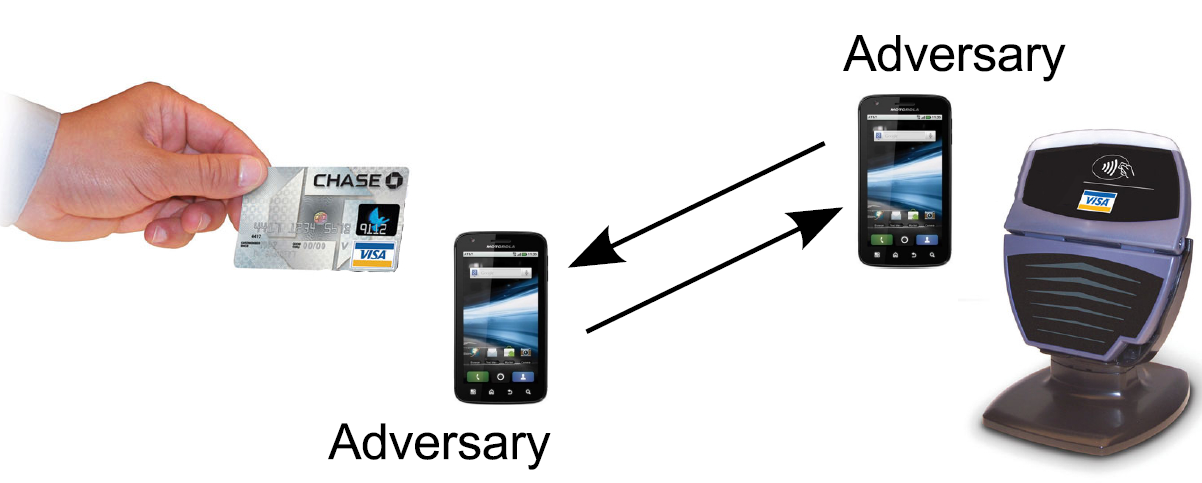
\includegraphics{img/relay-attack}
\end{figure}
\paragraph{Note:} The do-ability of the Relay attack depends on the timer
between the prover and the verifier. Usually the timer is not tight, by default
its 5ms but it can be extend by the prover.


\begin{description}
    \item[Distance Bounding] A distance bounding is a process whereby one party
    assured:
    \begin{itemize}
        \item Of the identity of a second party,
        \item That the latter is present in the neighborhood of the verifying
        party, at some point in the protocol
    \end{itemize}
\end{description}
\paragraph{Note:} Distance bounding protocol does not avoid relay attacks, if
adversary inside the area of coverage.

Measurement of the distance can be done in different ways:
\begin{itemize}
    \item With the GPS
    \item The strength of the received signal  (RSS)
    \item Round Trip Time (RTT)
\end{itemize}

\subsection{Protocol Analysis}
\begin{description}
    \item[Mafia Fraud] A mafia fraud is an attack where an adversary defeats a
    distance bounding protocol using a man-in-the-middle (MITM) between the
    reader and an honest tag located outside the neighborhood.
    \item[Terrorist Fraud] A terrorist fraud is an attack where an adversart
    defeats a distance bounding protocol using a man-in-the-middle (MITM)
    between the reader and dishonest tag located outside of the neighborhood,
    such that the latter actively helps the adversary to maximize her attack
    success probability, without giving to her any advantage for future attacks
    \item[Distance Fraud] Given a distance bounding protocol, a distance fraud
    is an attack where a dishonest and lonely prover purports to be in the
    neighborhood of the verifier.
\end{description}

%%TODO Hancke and Kuhn's Protocol

\subsection{Comparison with Decision Theory}
%%NOT sure if we have seen this

\section{Privacy}
\subsection{Impact}
Compared to other technologies (video,GSM,\ldots), RFID has several issue
concerning privacy:
\begin{itemize}
    \item Tags cannot be switched-off
    \item Passive tags answer without the agreement of their bearers
    \item Easy to analyze the logs of the readers
    \item Increasing of the communication range
    \item Tags can be almost invisible
\end{itemize}
Privacy issues concerning RFID is being seriously considered by authorites.

\subsection{Information Meaningful by Itself}
Privacy issues appear when the data sent by the tag reveals information
intrinsic to the marked object or the holder of the object
\footnote{With MOBIB card, personal data are stored in the clear in the card}.

\subsection{Mitigating the Problem}
\begin{itemize}
    \item Kill command to destroy the tag
    \item Use a faraday cages or a blocker tags to
    avoid clandestine query.
    \item \ldots
\end{itemize}
The problem with these solutions is that they are not convenient.
\paragraph{Note:} Nowadays more and more data are collected, it is called
logphilia. But with all these data, information may eventually leak.

The consequence of these information's leakage must be evalutated:
\begin{itemize}
    \item Does all these data need to be store?
    \item Encryption of the sensitive data on the tag in the dtabases
    \item Authentication for accessing the data
    \item Establishing policies to define who can access the data
\end{itemize}

\section{Biometric Passport}
\subsection{Description}
\begin{itemize}
    \item An Machine Readable Zone is composed of two lines of 44 characters
    \item Numbers and punctuations not authorized in the name field
    \item Hyphens are replaced by a filler character ('<')
    \item Apostrophes and commas are omitted
    \item First and last names are separated by 2 filler characters
    \item White characters are replaced by filler characters
\end{itemize}

\paragraph{Check Digits Calculation}
Check digits are computed for each protecfields. They are calculated modulo 10
with continous repetitive weihting of 731
\begin{itemize}
    \item Letters are mapped to their corresponding numerical value:
    A=10, B=11, \ldots,Z=35, '<' = 0.
    \item From left to right, each numerical value is multiplied by the weight
    appearing in the same sequential position.
    \item The product of each multiplication is added modulo 10
\end{itemize}
Ex: Calculate the check digit of the document number "EH123456<".
\begin{table}[ht!]
    \centering
    \begin{tabular}{c|c|c|c|c|c|c|c|c|c|}
        Number & E & H & 1 & 2 & 3 & 4 & 5 & 6 & < \\
        & 14 & 17 & 1 & 2 & 3 & 4 & 5 & 6 & 0 \\
        \hline
        Weight & 7 & 3 & 1 & 7 & 3 & 1 & 7 & 3 & 1\\
        \hline
        $N\times W \mod{10}$ & 98 & 51 & 1 & 14 & 9 & 4 & 35 & 18 & 0\\
    \end{tabular}
\end{table}
$$ 98+51+1+14+9+4+35+18 = 230 $$
$$ 230 \mod 10 = 0 $$
The remainder of the division is the check digit 0.

\subsubsection{Technical facts about the passport}
\begin{itemize}
    \item Tag is passive, i.e no internal battery
    \item Tag has a microprocessor (public-key crypto)
    \item Official distance 10cm
    \item EEPROM capacity: 32KB (minimum)
\end{itemize}

\subsubsection{Passport Content}
\begin{itemize}
    \item UID is publicly available
    \item Publicly available data, possibly after authentication
    \begin{itemize}
        \item Some data groups (DG)
        \item List of data groups on the considered passport (COM)
        \item Cryptographic material signature and hashes (SOD)
    \end{itemize}
    \item Data never supplied by the tag
    \begin{itemize}
        \item Two symmetric key $K_{ENC},K_{MAC}$ (can be retrieved from MRZ)
        \item One private key $K_{pr}$ (protected memory)
    \end{itemize}
\end{itemize}

\subsection{Protection Mechanisms}
\begin{figure}[ht!]
    \centering
    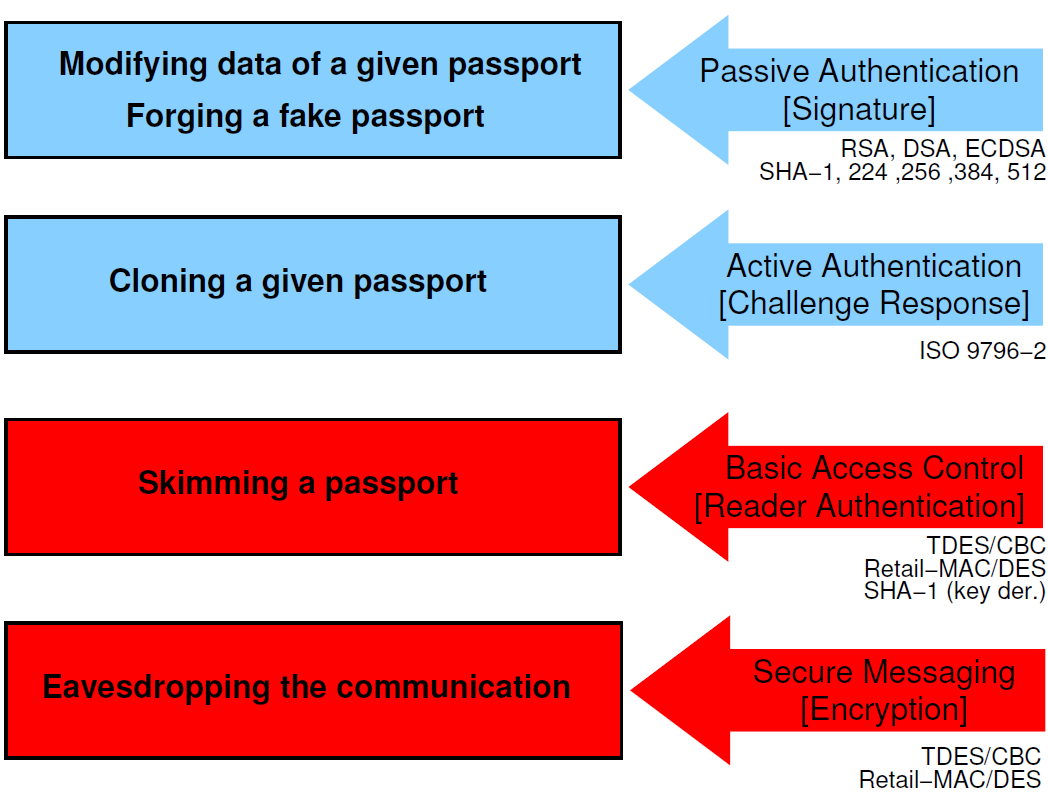
\includegraphics[scale=0.5]{img/e-passport}
\end{figure}

\subsubsection{Passive Authentication}
\begin{figure}[ht!]
    \centering
    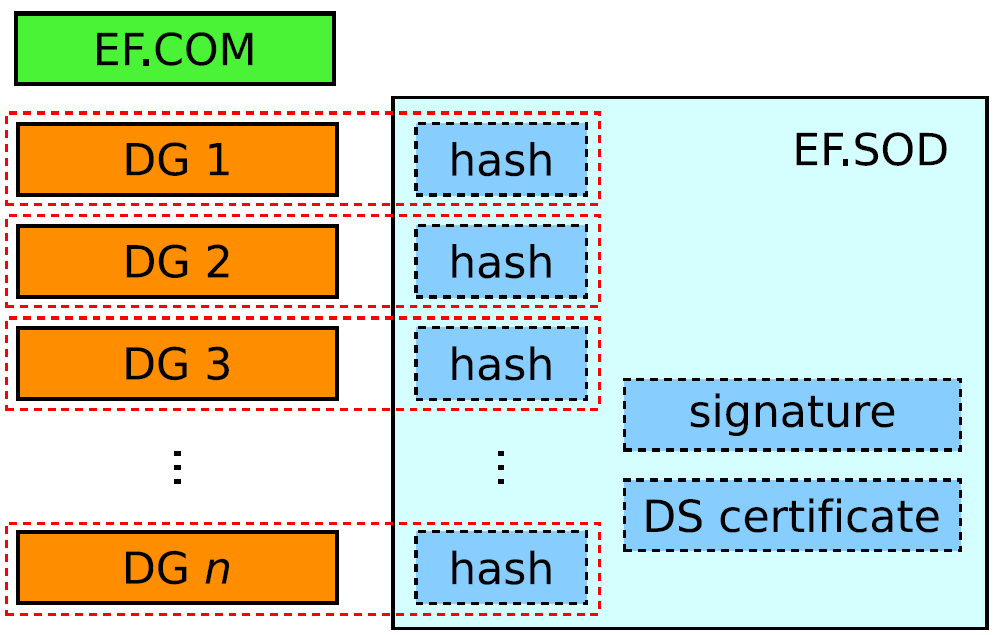
\includegraphics[scale=0.5]{img/passive-authentication}
\end{figure}

\begin{itemize}
    \item Passive authentication is a mandatory security mechanism, it proves
    that the file EF.SOD and LDS are authentic and not modified.
    \item EF.SOD contains the hash value of each present DG, and signature
    calculated by the issuing State over values.
    \item The signature can be checked using the Document Signer (DS) X.509
    certificate. (available from EF.SOD)
    \item The DS certificate can be checked using the Country Signing CA (CSCA)
    X.509 cerficate.
    \begin{itemize}
        \item The ICAO PKD does not publish the CSCA certificates
        \item CSCA certificates and revocation lists should be exchanged
        according to bilateral agreements
    \end{itemize}
\end{itemize}

\paragraph{Recommandations} According to DOC 9303:
\begin{itemize}
    \item The passive authentication should use RSA,DSA or ECDSA for the
    signature schemes
    \item SHA-1,SHA-2 for the hash algorithm
    \item CSCA keys should be renewed every three to five years and the DS
    keys every three months
\end{itemize}

\subsubsection{Active Authentication}
%%TODO add skecth
\begin{itemize}
    \item The active authentication is an optional security mechanism
    \item Aim is to prove the EF.SOD belongs to the authentic ePassport, i.e
    it is not a cloned one
    \item Two-pass CR protocol ISO 9796i\text{-}2 Digital Signature Scheme 1
    \item ePassport's public key is stored in DG15
\end{itemize}

The active authentication should rely on RSA,DSA or ECDSA and minimum sizes for
the security parameters should be 1024 bits, 1024 and 160 bits, and 160 bits,
respectively.
%%TODO example wih RSA/SHA1

\subsubsection{Access Control and Secure Messaging}
\begin{figure}[ht!]
    \centering
    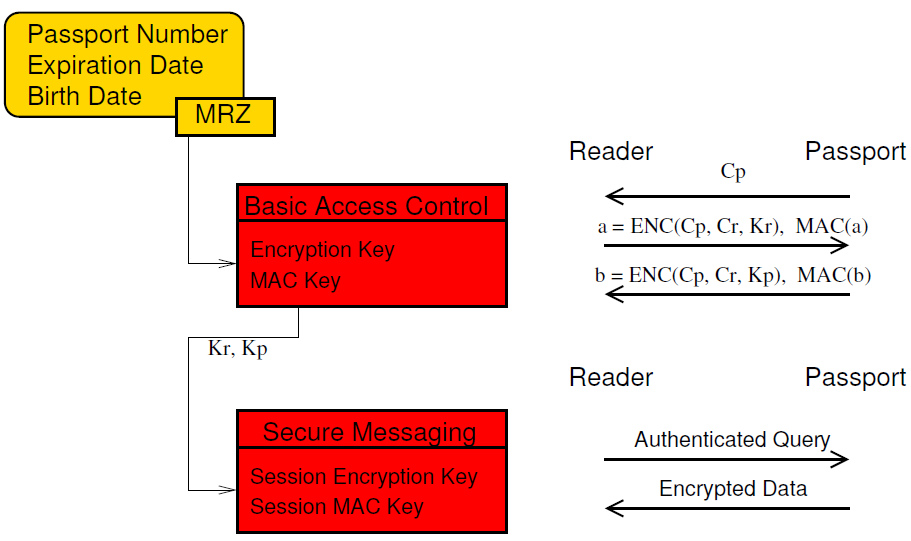
\includegraphics[scale=0.5]{img/access-control}
\end{figure}
\begin{itemize}
    \item Three-pass CR protocol according to ISO 11770\text{-}2 Key Establishment
    Mechanism 6, 2-key 3DES as block cipher
    \item Nonces should be 8-byte long
    \item Encryption done using 3DES in CBC mode with zero-IV according to
    ISO 11568\text{-}2
    \item A cryptographic checksum is calculated over: ISO 9797\text{-}1 MAC
    Algorithm 3 (i.e Retail-MAC), based on DES, zero-IV, ISO 9797\text{-}1 Padding
    Method 2
    \item Encryption and MAC keys derived from the MRZ using SHA-1
\end{itemize}

\paragraph{Key Derivation}
\begin{enumerate}
    \item Set $ K_{seed} = trunc_{16}(SHA-1(MRZ\_info))\quad or\ (K_r \oplus K_p)$
    \item Set $ D = K_{seed}||00000001 $
    \item Compute $ H = SHA-1(D) $
    \item First 16 bytes of H are set to the 2-key 3DES $ K_{ENC} $
    \item Set $ D = K_{seed}||00000002 $
    \item Compute $ H = SHA-1(D) $
    \item First 16 bytes of H are set to the 2 DES keys $K_{MAC} $
    \item Adjust the parity bits of the DES keys
\end{enumerate}

\subsection{Weaknesses}
BAC keys are derived from the MRZ, especially date of birth, date of expiry,
passport number. But passport numbers are usually not random. DOB and DOE are
neither random.

\begin{itemize}
    \item Relay Attacks: Passport is based on ISO 14443, so it can require to
    increase the timeouts.
    \item Evidence of Presence: Abuse the active authentication which can be
    doable without passing the BAC
    \item Chain og Trust: If the root certificate cannot be verified, making a
    fake passport is quite easy
\end{itemize}

\end{document}
